%!TEX root = main.tex
\section{System}
\subsection{System Architecture}

%We have implemented \system\ as a web-based tool on top of a a PostgreSQL database.

\begin{center}
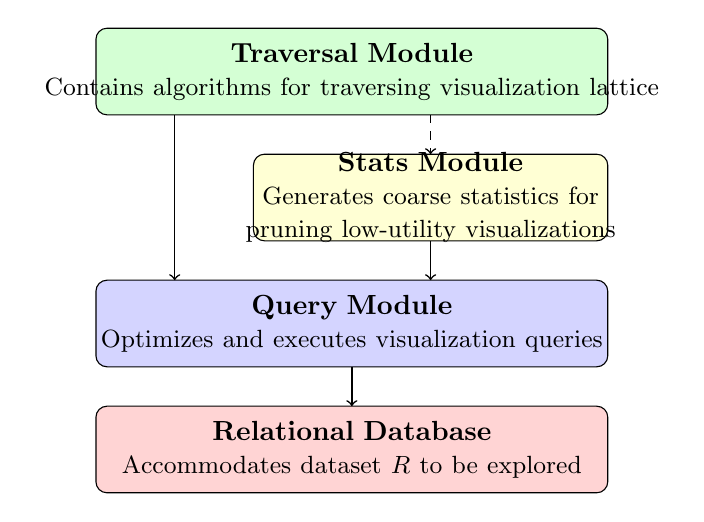
\begin{tikzpicture}
    \filldraw [fill={rgb:red,1;white,5}, rounded corners=4pt] (0, 0) rectangle (6.5, 1.1) node[pos=.5, align=center, text width=8cm] {\textbf{Relational Database}\\ {\small Accommodates dataset $R$ to be explored}};
    \filldraw [fill={rgb:blue,1;white,5}, rounded corners=4pt] (0, 1.6) rectangle (6.5, 2.7) node[pos=.5, align=center, text width=8cm] {\textbf{Query Module}\\ {\small Optimizes and executes visualization queries}};
    \filldraw [fill={rgb:yellow,1;white,5}, rounded corners=4pt] (2, 3.2) rectangle (6.5, 4.3) node[pos=.5, align=center, text width=5cm] {\textbf{Stats Module}\\ {\small Generates coarse statistics for pruning low-utility visualizations}};
    \filldraw [fill={rgb:green,1;white,5}, rounded corners=4pt] (0, 4.8) rectangle (6.5, 5.9) node[pos=.5, align=center, text width=8cm] {\textbf{Traversal Module}\\ {\small Contains algorithms for traversing visualization lattice}};
    \draw [->, line width=0.2mm] (1, 4.8) -- (1, 2.7);
    \draw [->, dashed, line width=0.2mm] (4.25, 4.8) -- (4.25, 4.3);
    \draw [->, line width=0.2mm] (4.25, 3.2) -- (4.25, 2.7);
    \draw [->, line width=0.2mm] (3.25, 1.6) -- (3.25, 1.1);
\end{tikzpicture}
\end{center}


\subsection{Algorithms}
\subsection{User Interaction}
\subsection{Basic Usage Scenario}
\subsection{Assistive tools for visualizing large lattices}